\documentclass[11pt,a4paper]{article}
\usepackage[margin=2.4cm]{geometry}
\usepackage{graphicx}
\usepackage{booktabs}
\usepackage{amsmath}
\usepackage{amssymb}
\usepackage{array}
\usepackage{microtype}
\usepackage[hidelinks]{hyperref}
\usepackage{parskip}

\title{\vspace{-1.5cm}Per-system performance, the pseudo-labels, and a per-class design\\[2pt]
\large For the meeting on 2 October 2026}
\author{Brhanu Atsbaha}
\date{29 September 2026}

\begin{document}
\maketitle
\vspace{-0.7cm}

\section*{What this answers}

This covers the four things you asked for in the September meeting, plus the baseline question: how
each system performs on the hand-annotated pictures, what the other systems say about the teacher's pseudo-labels, a hand
inspection of those labels, a design for agreement at the image/class level, and which published
baseline each result is measured against. It closes with
annotation progress and one point about conformal risk control I would like to settle in writing.

\section{One model, and which classes}

\textbf{One model, not eight.} The detector is a single multi-class YOLOv11 trained jointly. At the
frequencies these classes have in the archive, per-class detectors would not be trainable: the whole
hand-annotated set contains 9 pictures with a vehicle and 8 with a hat.

\textbf{The class list, frozen.} Three lists were in circulation, which is my fault for not fixing one
earlier. The rater's list and the detector's list agree on eight object classes and differ on two: the
rater drew furniture and hat, the detector was trained for horse and clothing. In 300 hand-annotated
pictures there is not one horse or clothing box, and the detector cannot emit furniture or hat at all.
I therefore propose freezing the eight classes both lists share:

\begin{center}
person \quad child \quad animal \quad building \quad weapon \quad vehicle \quad tree \quad text
\end{center}

and keeping the five scene classes (teaching, family, playing, landscape, drawing) separate, as scene
labels rather than objects. Furniture and hat stay measurable for the two systems that can score any
class from a prompt, and are reported separately where they appear.

\section{The baselines}

You asked which baseline the results are compared against. Each of the thesis's three questions
now has a published baseline, run on this archive's own pictures with the same scoring as everything
else in this document.

\begin{table}[h]
\centering
\small
\begin{tabular}{>{\raggedright\arraybackslash}p{3.1cm}>{\raggedright\arraybackslash}p{4.3cm}>{\raggedright\arraybackslash}p{6.6cm}}
\toprule
Question & Baseline & Result on this archive \\
\midrule
Detecting objects in historical illustrations &
Kim, Im and Mandl, \emph{Object Detection in Historical Images: Transfer Learning and Pseudo
Labelling}, JOCCH 2024 --- the paradigm this detector follows; its starting point is a COCO-pretrained
detector used as-is &
On the 300 pictures, AUROC for person, animal, vehicle, furniture: COCO detector as-is 0.79, 0.74,
0.75, 0.69; after adaptation by pseudo-labelling 0.87, 0.81, 0.55, --- (it cannot emit furniture);
LLaVA asked per class 0.94, 0.93, 1.00, 0.92. \\
\addlinespace
Detecting the pipeline's errors &
Hendrycks and Gimpel, \emph{A Baseline for Detecting Misclassified and Out-of-Distribution Examples
in Neural Networks}, ICLR 2017 --- a model's own confidence &
On the 249 held-out test pictures, confidence scores AUROC 0.872 against 0.860 for the disagreement
signal. The thesis's negative answer to RQ1 is precisely a loss to this baseline. \\
\addlinespace
Approving pictures automatically under a risk target &
Geifman and El-Yaniv, \emph{Selective Classification for Deep Neural Networks}, NIPS 2017 ---
approval with a guaranteed error rate among approved pictures; and random review &
Same score, same 500 splits. At the same stated target of 0.05, selective classification approves
16\% and conformal risk control 63\%, because the former bounds the stricter quantity with 95\%
confidence. At the same approval rate (about 62\%) both give about 2.9\% error among approved
pictures and catch about 90\% of errors. Random review catches errors in proportion to the pictures
reviewed. \\
\bottomrule
\end{tabular}
\caption{One published baseline per question.}
\end{table}

Two consequences. Adaptation by pseudo-labelling is worth its cost for person and animal but not for
vehicle, and a zero-shot vision-language model beats both. And conformal risk control is not a better
ranker than the published alternative --- it gives a different, weaker guarantee in exchange for more
automatic approval, which is how the thesis should present it.

\section{Each system on the 300 hand-annotated pictures}

Every system is scored per class. Where a system needs a yes/no cut-off, the cut-off is chosen by
five-fold cross-validation, so no picture is judged with a threshold fitted on itself. Each class is
also compared against answering ``yes'' for every picture, which for rare classes is a surprisingly
strong baseline.

\begin{table}[h]
\centering
\small
\begin{tabular}{lccc}
\toprule
System & Mean AUROC & Mean F1 & F1 with its own fixed rule \\
\midrule
LLaVA-OneVision (one question per class) & \textbf{0.91} & \textbf{0.65} & 0.57 \\
Fusion of the three & 0.90 & 0.60 & --- \\
SigLIP (one prompt per class) & 0.85 & 0.51 & --- \\
Detector (top box confidence) & 0.62 & 0.35 & 0.24 \\
Answering yes for every picture & --- & 0.28 & --- \\
\midrule
Kosmos-2.5, text class only & 0.55 & 0.38 & 0.38 \\
\bottomrule
\end{tabular}
\caption{Averages over the eight frozen classes, 300 pictures. The fixed rules are the detector's
confidence 0.25, LLaVA's P(yes) 0.5 and three or more words read by Kosmos.}
\end{table}

\begin{figure}[h]
\centering
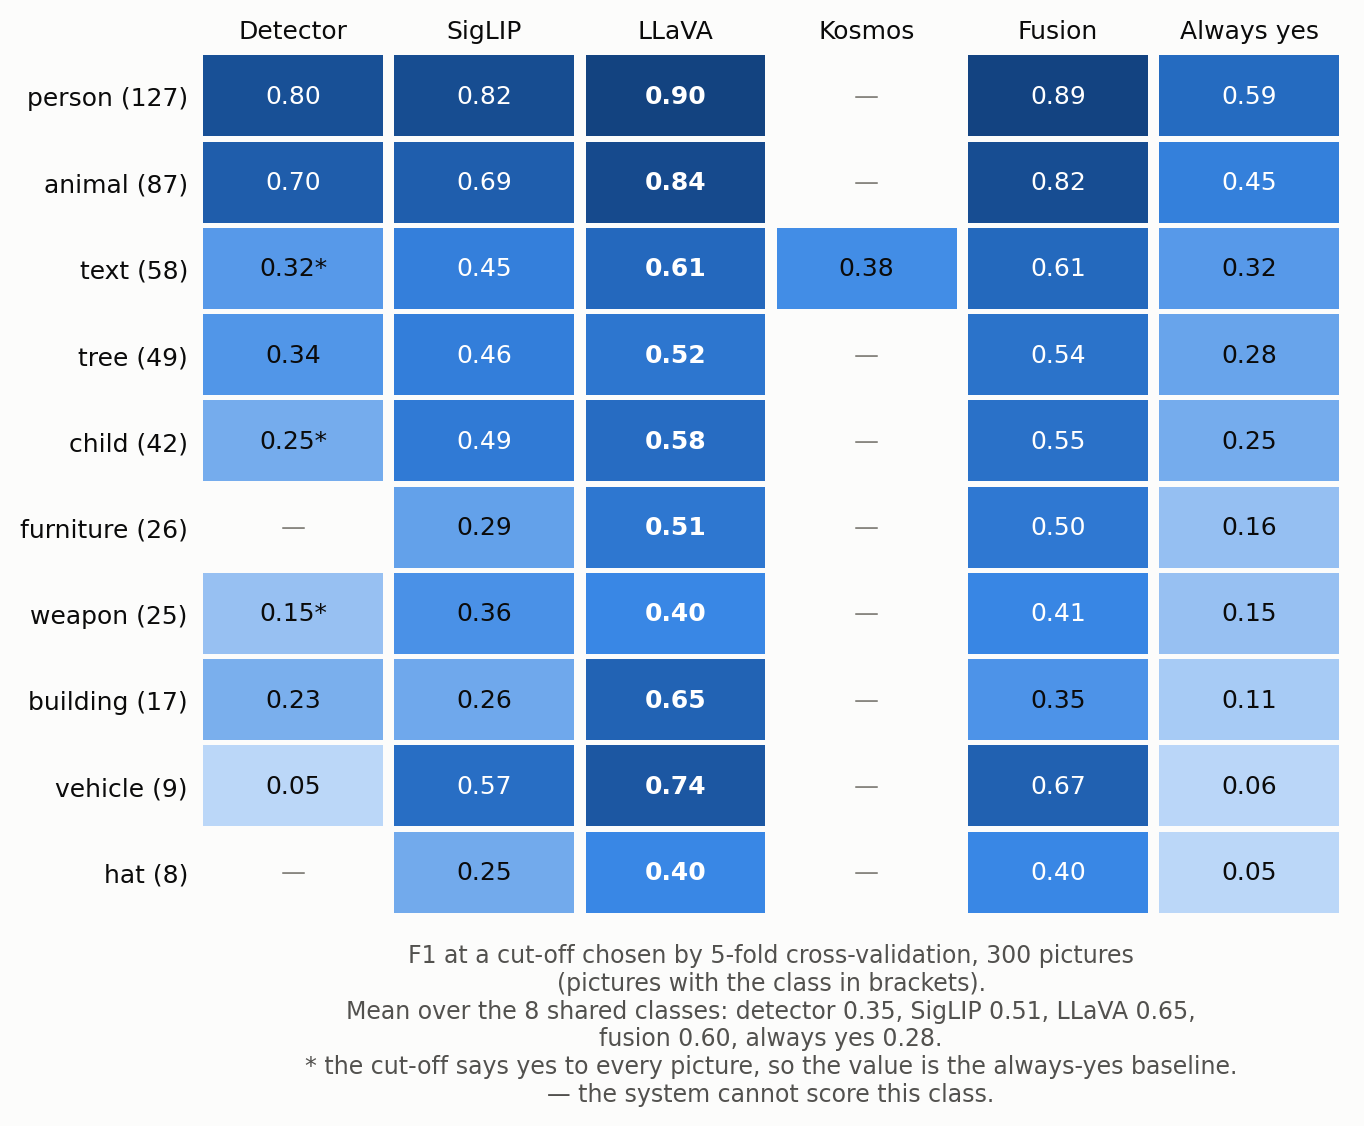
\includegraphics[width=0.92\textwidth]{../latex_assets/b1/b1_f1_by_class_and_system.png}
\caption{F1 by class and system. The last column is the always-yes baseline for that class.}
\end{figure}

\paragraph{The detector} works for person (F1 0.80) and animal (0.70) and adds nothing elsewhere. For
child, weapon and text its best cut-off is to answer yes to every picture, and it never emits a text
box at any confidence. Its box-level accuracy on these pictures is mAP50 0.146, and 0.111 on the 164
pictures that were not in its training split --- 136 of the 300 were, which is a leak I inherited and
now report around rather than through.

\paragraph{SigLIP} ranks every class well (AUROC 0.75--0.93) but its raw scores are not calibrated:
most pictures sit near zero, so a fixed threshold is meaningless and the cross-validated cut-offs land
mid-range. Calibration, not capability, is what limits it.

\paragraph{LLaVA-OneVision} is the strongest system on every class once it is asked one yes/no question
per class and read through the probability of ``yes'' rather than through free text. The deployed
four-question form could not do this. Two different phrasings of the same question agree on 95.7\% of
decisions, and the result holds on the 200 pictures that played no part in choosing the phrasing.

\paragraph{Kosmos-2.5} reads text but barely separates pictures that contain text from pictures that do
not (AUROC 0.55), because much of its output is repetition. It is a source of negative evidence, not a
per-class rater --- which is why the agreement design below has three raters, not four.

\paragraph{Print quality} does not explain the failures. On the 52 pictures the rater marked blurry or
faded, no system is worse than on the 248 clear ones (LLaVA 0.66 on the blurry or faded ones, 0.65 on the clear).

\section{What the other systems say about the pseudo-labels}

Two pseudo-label sets exist. Neither records what its class ids meant when written, so I tested them
the way you suggested: by asking what the other systems see where the teacher placed a label. SigLIP
and LLaVA never saw either set, so their votes are independent; the detector's are not, since it was
trained on one of them.

\begin{figure}[h]
\centering
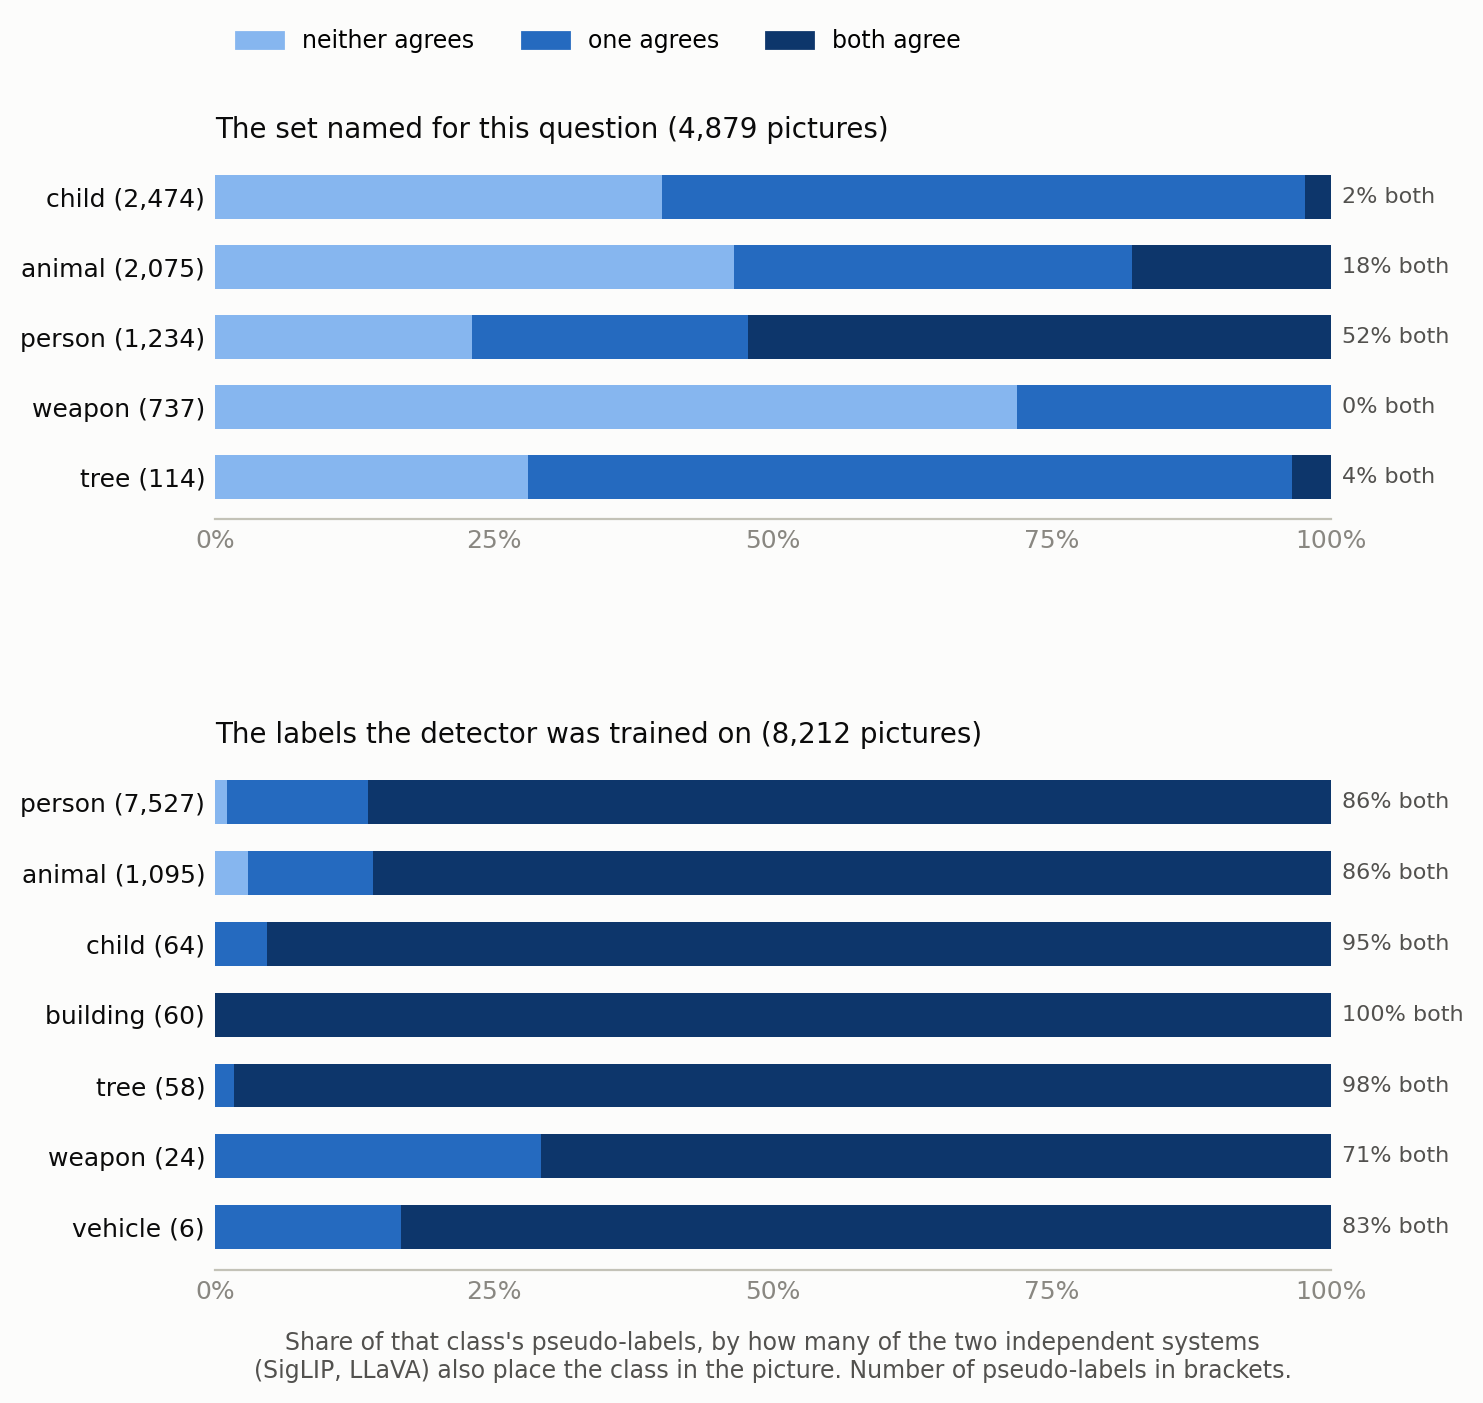
\includegraphics[width=0.92\textwidth]{../latex_assets/b2/b2_agreement_by_class.png}
\caption{How many of the two independent systems agree with each pseudo-label.}
\end{figure}

On the labels the detector was trained on, both independent systems confirm 71--100\% of pseudo-labels
and neither confirms at most 3\%. Those same votes also identify the disputed class ids: the ids read
as horse, clothing and animal, which is the detector's original training order and not the order now
recorded in the dataset file. The text class was never emitted at all.

On the other set --- the one with roughly three thousand labelled pictures --- agreement collapses: both
systems confirm 52\% of person labels, 18\% of animal, 2\% of child and none of the 737 weapon labels,
and neither confirms between 23\% and 72\% depending on class. I would not build on that set without
re-generating it.

\section{Hand inspection of the pseudo-labels}

Twenty boxes were drawn stratified across class ids rather than at random (random returns persons: one
class accounts for 88\% of all 18,969 boxes over 8,212 pictures and 1,189 volumes, and one class is
never emitted). Each was judged by hand with the box drawn in its picture; nineteen are done.

All nineteen boxes were judged well placed, and for every class id whose name never changed, the
content matched the name. The three ids whose names were rewritten after training tell the story:

\begin{table}[h]
\centering
\begin{tabular}{llll}
\toprule
Class id & Name at training & Name in the dataset file now & Hand judgement \\
\midrule
9 & animal & furniture & animal (4 of 4) \\
7 & clothing & text & child (3 of 3) \\
2 & horse & animal & animal (3), horse (2) \\
\bottomrule
\end{tabular}
\caption{The disputed class ids, judged by hand.}
\end{table}

The names written into the dataset file after training are wrong for two of the three ids, which
confirms what the independent systems showed in Section 4 --- with one correction: the id trained as
``clothing'' marks children, not garments. Under the frozen eight-class list this resolves cleanly:
horses merge into animal, and the clothing id is not one of the eight.

One figure from my own earlier notes needs correcting: the student's object count is zero on 2,882
pictures (23.8\%), not on the 10,707 I previously wrote down; that number came from a different
quantity.

\paragraph{Whose failure are the misses?} On the 137 hand-annotated pictures that also carry the
teacher's pseudo-label, the student misses 128 hand-drawn objects. For 126 of them the teacher's
label never contained the object; only 2 were in the label and went unlearned. The teacher labelled no
child (0 of 32), weapon, building, vehicle or text on these pictures, and the student copies it closely,
errors included (23 wrong person labels from the teacher, 24 from the student). Across the archive the
student finds nothing on 2,882 pictures, but only 17 of those were in its training data. The fix
therefore belongs in the teacher and in which pseudo-labels are kept, not in longer or reweighted
training.

\paragraph{A first rebuild.} I replaced the teacher accordingly. GroundingDINO, prompted with the eight
class names and kept only where LLaVA confirms the class, labelled 11,028 training pictures --- none of
the 300 evaluation pictures and none of the risk-control calibration or test pictures. A YOLO11m student
trained from the same COCO starting point reaches a mean box AP50 of 0.205 on the human boxes, against
0.123 for the deployed student; on the 164 pictures neither student trained on, 0.186 against 0.106.
The largest gains are on the classes the old teacher never labelled (building 0.05 to 0.23, vehicle 0 to
0.23, child 0.05 to 0.13). The teacher itself reaches 0.283, so the student has not yet caught up with
it.

\section{Human agreement, and what it limits}

Two people have independently rated scene categories on 124 of the audit pictures. Overall agreement
is Cohen's $\kappa = 0.34$ (95\% CI 0.21--0.45), and per category:

\begin{table}[h]
\centering
\begin{tabular}{lccc}
\toprule
Category & $\kappa$ & 95\% CI & Can it carry a result? \\
\midrule
landscape & 0.81 & 0.63--0.94 & yes \\
family & 0.43 & $-0.02$--0.80 & only just; 3 and 6 positives \\
drawing & 0.26 & 0.13--0.40 & no \\
playing & 0.25 & 0.02--0.47 & no \\
teaching & $-0.01$ & $-0.03$--0.00 & no \\
\bottomrule
\end{tabular}
\caption{Per-category agreement between two raters on 124 pictures.}
\end{table}

This is a limit on what any scene result can claim, and I would rather state it than report metrics
against labels two people do not agree on. A second rating of 150 further pictures is being collected
to put intervals on this.

\section{A design for agreement at the image/class level}

For sign-off before I build it:

\begin{enumerate}
\item Each system emits a score for every class on every picture. This now exists for all 12,110
      pictures and three systems; Kosmos is excluded as above, which makes three raters and three pairs.
\item Agreement per picture and class is $1 - |s_1 - s_2|$, as you formulated it, but only after the
      scores are put on a common scale. As they stand, one system's scores sit near zero and another's
      spread over the whole range, so the raw difference would measure scale rather than disagreement.
      I propose calibrating each system per class on the labelled pictures and reporting the
      rank-based version alongside.
\item Aggregations: per image and class, per class, per image, per model pair, and one global mean.
\item Chance-corrected agreement per class: pairwise Cohen's $\kappa$ for each pair and Fleiss'
      $\kappa$ across all three at once, with prevalence and a prevalence-adjusted value beside them,
      since at these base rates high raw agreement produces near-zero $\kappa$.
\item The comparison I find most interesting: machine agreement against the human agreement above. Do
      the models agree with each other more or less than two people do?
\end{enumerate}

A first look on the rank scale already exists. Fleiss' $\kappa$ across the three systems runs from 0.68
for person to 0.01 for vehicle. On the 300 pictures, the two strongest systems agree with each other
more than either agrees with the human rater for child, building, weapon and tree (for text the two
are level, 0.477 against 0.474) --- so for those classes, agreement between systems is not evidence
that they are right.

\section{The class-level test of RQ1}

Your per-class formulation reopened RQ1, so I tested it in the form that could have changed the answer.
Before running anything I fixed, in a dated and committed pre-registration, the five signals, the two
evaluation sets, the metric and the decision rule: if per-class disagreement beats plain confidence on
the 300 hand-annotated pictures with a DeLong 95\% interval entirely above zero, RQ1 becomes a qualified
yes; otherwise it stays no. Per-class scores were calibrated by Platt scaling, cross-fitted so that no
picture is scored by a calibration that saw it.

\begin{table}[h]
\centering
\small
\begin{tabular}{lccc}
\toprule
Signal (AUROC for the pipeline's errors) & 300 pictures & 164 not in training & Test split \\
\midrule
Per-class disagreement (the one tested) & 0.378 & 0.467 & 0.366 \\
Per-class entropy & 0.286 & 0.402 & 0.252 \\
Global disagreement & 0.484 & 0.458 & 0.578 \\
Deployed disagreement signal & 0.799 & 0.646 & 0.860 \\
Plain confidence & \textbf{0.825} & \textbf{0.728} & 0.720 \\
\bottomrule
\end{tabular}
\caption{The pre-registered test: 72 errors among the 300 pictures, 61 among the 164, 70 in the test split.}
\end{table}

The registered difference, per-class disagreement minus confidence, is $-0.448$ (DeLong 95\% CI
$-0.541$ to $-0.354$), so RQ1 stays no --- now at two levels of detail rather than one. The reason is
concrete: 65 of the 72 errors are missed scenes, on pictures with fewer objects (0.9 annotated classes
against 1.53 on correct ones). There all three systems score every class low and so agree; the errors sit
exactly where agreement is highest.

\section{What the Tier-1 agents actually measured, and a corrected re-run}

Working through the per-class formulation raised a question about the four Tier-1 signals themselves,
and the answer changes how the pipeline should be described. Reading the stored signal table against
the code that produced it establishes three things, each of which holds on every one of the 12,110
pictures with no exceptions:

\begin{itemize}\itemsep2pt
  \item The spatial object signal is not the detector's output. The distilled student returned no boxes
        at all, so a fallback supplied the visual-question-answering object count instead:
        $A^{\text{object}} = \min(\text{count}/3,\,1)$, which takes four values.
  \item The visual-reasoning signal is an indicator of that same count:
        $A^{\text{vlm}} = \mathbb{I}[A^{\text{object}} > 0]$, two values.
  \item The agreement signal is arithmetic over the other two,
        $A^{\text{agree}} = 1 - |A^{\text{object}} - A^{\text{vlm}}|$. No picture in the archive carries a
        measured agreement score.
\end{itemize}

The scene signal has a separate defect. It was read from a softmax over five scene prompts, which is a
forced choice among scene types and so cannot express the absence of a scene; its minimum over the
corpus is $0.2956$. Against human scene-presence labels that channel scores AUROC $0.417$, below
chance at the quantity it names, while the sigmoid channel computed in the same pass scores $0.775$
(paired difference $0.358$, 95\% CI $0.299$ to $0.415$).

\paragraph{Why this limits the design rather than one number.} With four, two and two reachable values,
the three measured signals realise eight distinct joint states. Any function of them --- any weighting,
any nonlinearity, any learned model --- is constant inside a state and can take at most eight values.
The disagreement signal does take exactly eight, with 34\% of the archive at exactly zero. The Tier-1
vector carries at most three bits per picture, which is why the pipeline reduces in practice to a
scene/no-scene decision rather than to the distinct agent roles the design specifies.

\paragraph{The corrected re-run.} I re-ran the pipeline end to end with each agent emitting the output
its specification promises, keeping scene presence as the target and the fusion weights unchanged:
the rebuilt detector's per-class confidences over the eight frozen classes; SigLIP's sigmoid over the
five scene prompts; the vision-language model's per-class $P(\text{yes})$ read from first-token
logprobs. The agreement term is dropped. Because the deployed fusion averages a count, a flag and a
binary answer, its spread partly measures how those scales were normalised rather than models
disagreeing; here each agent keeps its own vector and is mapped to a probability of scene presence by
a logistic fit on the training split alone, so the three estimate the same quantity on the same scale.
No agent sees another's features, the conformal threshold is calibrated on the calibration split, and
everything below is the held-out test partition ($n=249$).

\begin{table}[h]
\centering
\small
\begin{tabular}{lccc}
\toprule
 & Scene AUROC & Test error rate & Distinct uncertainty values \\
\midrule
Deployed & 0.779 & 0.281 & 8 \\
Corrected, deployed detector & 0.783 & 0.153 & 249 \\
Corrected, rebuilt detector & 0.826 & 0.153 & 249 \\
\quad + absence router & \textbf{0.854} & \textbf{0.145} & 249 \\
\bottomrule
\end{tabular}
\caption{The committed test split of 249 pictures. Both arms scored with the same Level-2 fusion,
$0.6$ object $+\,0.2$ scene $+\,0.2$ VLM, and the same decision threshold. How much of this survives
other splits and another labeller is the subject of the last part of this section.}
\end{table}

The agents are now separately informative instead of three views of one answer: alone on the test
partition, the object agent reaches AUROC $0.828$, the visual-reasoning agent $0.822$ and the scene
agent $0.718$.

\paragraph{What it does to RQ1.} It leaves the answer unchanged and supports it better. With agents
that work, plain confidence predicts the pipeline's errors at $0.826$ against disagreement's $0.780$.
In the deployed system the ordering looks reversed --- disagreement $0.860$ against confidence
$0.720$ --- but that comparison is against a confidence baseline computed from an eight-valued step
function. The negative answer to RQ1 therefore does not depend on the weak component; correcting the
component leaves it standing.

\paragraph{Letting the scene agent say ``none of these''.} Five prompts that all name a scene type
cannot report that a picture is none of them, and that is the pipeline's dominant error: calling a
non-scene a scene. The negative-control audit established what the true negatives actually are ---
printed text, sheet music, ornament, blank and title pages, tables of numbers, maps --- and SigLIP
scores those prompts in the same pass. Giving the scene agent that one extra number raises scene
ranking from $0.826$ to $0.854$ on the committed split, and lowers the error rate from $0.153$ to $0.145$.

\paragraph{What the triage score should be.} The deployed triage score is disagreement. In every
corrected variant plain confidence predicts the pipeline's errors better, and triage is where that
matters, since it decides which pictures a person never sees. Scoring the same guarantee by
confidence instead, on the test partition:

\begin{table}[h]
\centering
\small
\begin{tabular}{lccc}
\toprule
Pictures approved automatically & $\alpha=0.05$ & $\alpha=0.10$ & $\alpha=0.15$ \\
\midrule
Deployed & 30.9\% & 60.2\%$^\dagger$ & 79.1\% \\
Corrected, rebuilt detector & 65.1\% & 79.9\% & \textbf{97.6\%} \\
Corrected + absence router & \textbf{67.1\%} & \textbf{82.7\%} & \textbf{97.6\%} \\
\bottomrule
\end{tabular}
\caption{Triage scored by confidence rather than disagreement. Every bound is satisfied for the
corrected pipelines; scored by disagreement instead, the pipeline with the absence router exceeds the
two tightest targets.
$^\dagger$the one target the deployed pipeline exceeds.}
\end{table}

The deployed pipeline gets \emph{worse} under confidence, not better, which is the same ceiling
again: its confidence is an eight-valued step function, so there is no finer threshold to find. The
recommendation only works on signals that are continuous.

\paragraph{The risk guarantee, checked properly.} On the committed split, triage scored by disagreement
exceeds the risk target at $\alpha = 0.01$ and $0.02$ once the absence router is added. That is not by itself evidence against the
guarantee: conformal risk control bounds the risk in expectation over draws of the calibration set,
not the risk of any one split. Drawing the split again 200 times over the 1,250 labelled pictures,
with books partitioned 60/20/20 so that no book is ever on two sides, the mean realised risk sits
below the target at every one of the five targets, for both pipelines.

\begin{table}[h]
\centering
\small
\begin{tabular}{lcccc}
\toprule
Target & \multicolumn{2}{c}{Mean realised risk} & \multicolumn{2}{c}{Auto-approved} \\
\cmidrule(lr){2-3}\cmidrule(lr){4-5}
 & Deployed & Corrected & Deployed & Corrected \\
\midrule
0.01 & 0.0071 & 0.0091 & 39.9\% & 25.6\% \\
0.02 & 0.0127 & 0.0189 & 51.8\% & 40.4\% \\
0.05 & 0.0156 & 0.0486 & 61.1\% & 60.2\% \\
0.10 & 0.0218 & 0.0998 & 62.1\% & \textbf{81.9\%} \\
0.15 & 0.0786 & 0.1375 & 70.7\% & \textbf{94.7\%} \\
\bottomrule
\end{tabular}
\caption{200 book-disjoint redraws. The guarantee holds for both pipelines; what differs is how much
of the risk budget each can spend.}
\end{table}

The difference worth reporting is not compliance but efficiency. The corrected pipeline's realised
risk tracks its target closely, which is what a guarantee that is being used looks like, and it buys
much more automation: $81.9\%$ of pictures approved at a target of $0.10$ against the deployed
pipeline's $62.1\%$. The deployed pipeline leaves most of its budget unspent --- $0.0218$ against a
target of $0.10$ --- because eight distinct uncertainty values admit no finer threshold, so its
auto-approval cannot rise past roughly $62\%$ however much risk is permitted.

\paragraph{How much of this survives other splits and other labels.} The figures above come from
one split of 249 pictures. I redrew it 200 times, books partitioned 60/20/20, refitting the agents'
mappings and recalibrating the threshold on every draw:

\begin{table}[h]
\centering
\small
\begin{tabular}{lcc}
\toprule
 & Scene AUROC & Test error rate \\
\midrule
Deployed & 0.829 \,[0.770, 0.893] & 0.254 \,[0.176, 0.337] \\
Corrected & 0.852 \,[0.784, 0.917] & 0.155 \,[0.092, 0.224] \\
Corrected + absence router & 0.867 \,[0.811, 0.922] & 0.156 \,[0.092, 0.224] \\
\bottomrule
\end{tabular}
\caption{Mean over 200 book-disjoint redraws, with the 2.5th and 97.5th percentiles.}
\end{table}

One result is robust, in the sense that the interval over paired draws excludes zero: the corrected
pipeline with the absence router and confidence-scored triage approves more pictures than the deployed
pipeline at the same guaranteed risk --- by 15.8 points at $\alpha=0.05$ (95\% of draws 5.6 to 29.2),
27.7 at $0.10$ (14.4 to 39.3) and 26.8 at $0.15$ (3.5 to 44.3) --- and its realised risk sits at the
target within Monte Carlo error at every target. The rest is likely but not established at that level:
the gain in scene ranking over the deployed pipeline (positive in 87.0\% of draws), the gain in error
rate (93.5\%), the absence router's own contribution (88.5\%), and confidence over disagreement as the
triage score within the corrected pipeline (89.5\%). The committed split overstated the ranking gain;
it happened to be a hard split for the deployed pipeline ($0.779$ there, $0.829$ on average).

The hand-annotated pictures give a second check. Ninety of them, from 57 books, come from books the
corrected pipeline was never fitted or calibrated on. On those the deployed pipeline ranks better,
AUROC $0.929$ against $0.888$ (difference $-0.037$, book-bootstrap interval $-0.122$ to $+0.035$), while
the error rates are indistinguishable ($0.211$ against $0.189$). Part of the reason is the target
itself: where a picture carries both labels, the rater and the scene pool agree on 82.2\% of 197
pictures, Cohen's $\kappa = 0.41$, and the rater is stricter about what counts as a scene --- of the
41 pictures they call no scene, the pool calls 22 a scene. The corrected mappings learned the pool's
definition. With labels this far apart, differences of a few hundredths in AUROC are within what
label disagreement alone produces. I tested that explanation directly on the 197 pictures that carry
both labels, scoring the corrected pipeline out of fold so that no picture is scored by a fit that saw
its book. The order flips with the label set: against the scene pool's labels the corrected pipeline
ranks better ($0.861$ against $0.840$), against the second rater's the deployed one does ($0.818$
against $0.789$), and where the two labels agree the corrected one is slightly ahead ($0.908$ against
$0.897$). No interval excludes zero, so this supports the explanation rather than proving it, but it
rules out the stronger reading that the corrected pipeline is worse out of pool.

What I think the thesis can claim, then, is the operational result, stated for the pool's definition
of a scene: the corrected pipeline automates substantially more at the same guaranteed risk. That it
transfers to another labeller's definition is not shown, and I would not claim it.

\paragraph{A consequence for the heterogeneity precondition.} The thesis uses the effective rank of
the agents' signals, with a threshold of 2, as the precondition for disagreement to be informative, and
reports that Colibri passes it (2.17 over the three measured signals). On the corrected signals the
effective rank is $1.37$ ($1.67$ with the absence router): once each agent is a calibrated estimate of
the same quantity, the agents agree --- the object and vision-language agents correlate at $0.920$.
The deployed signals looked heterogeneous because they measured different, badly scaled things, not
because they carried independent evidence. Read as a quality check the threshold is backwards; read as
a guard on the disagreement path it is right, and it points the same way as the triage result above.

I would like your view on whether to report the corrected pipeline as the thesis's system, with the
deployed one as the audited starting point, or to keep the deployed pipeline as the object of study
throughout.

\section{Conformal risk control: one point to settle}

Conformal risk control needs three things: an exchangeable calibration set, a scalar score, and a loss
that is monotone in the threshold and bounded. It is not restricted to the outputs of a pretrained
language model. The method was introduced for image segmentation and multilabel classification, among
others:

\begin{itemize}
\item Angelopoulos, Bates, Fisch, Lei, Schuster, \emph{Conformal Risk Control}, ICLR 2024.
\item Bates, Angelopoulos, Lei, Malik, Jordan, \emph{Distribution-Free, Risk-Controlling Prediction
      Sets}, Journal of the ACM 68(6), 2021.
\end{itemize}

The triage score here satisfies all three conditions and is a function of all four systems rather than
one model's output. What I would concede in the same breath is the real limitation: the guarantee holds
relative to the calibration distribution, and our own cross-archive pilot shows that assumption failing
when the archive changes.

Two corrections to how I have been reporting it. First, the guarantee is about the average over
calibration draws, not about one split: repeating the publication-level split 500 times, the mean test
risk stays within the target at every level, while a single split exceeds it between 1\% and 31\% of the
time depending on the level. Reporting one split's pass or fail was misleading in both directions.
Second, the reported risk is the marginal one (5 errors over 249 test pictures); the quantity the text
described is the error rate among approved pictures (5 over 151). Both will be given separately.

\section{Annotation progress and the target}

Confirmed negatives in the labelled pool have grown from 196 to 319, of which 65 are in the held-out
test partition. The target is at least 80 there, which needs roughly 175 more pictures reviewed from a
randomly ordered block; that review is under way. Separately, rare classes are being searched three
ways at once --- clusters of the whole archive's embeddings, prompt-ranked candidates, and volumes that
appear to be single-content --- so that the yield per hour of each tactic can be compared rather than
assumed. Hand-picked pictures will be used for training and diagnosis only; the calibration and test
partitions stay randomly drawn, otherwise the risk figures stop meaning what they say.

\section*{What I would like from you}

\begin{enumerate}
\item Sign-off on the eight-class list and the five scene classes.
\item Sign-off on the agreement design in Section 7, in particular the calibration step.
\item Agreement that conformal risk control applies here, or your objection in writing so I can address
      it in the thesis.
\item A view on the weaker pseudo-label set: re-generate it, or proceed with the set the detector was
      trained on.
\end{enumerate}

\end{document}
